% !TEX encoding = UTF-8
% !TEX TS-program = pdflatex
% !TEX root = ../Tesi.tex
% !TEX spellcheck = it-IT

%************************************************
\chapter{Diagramma E-R}
\label{cap:diagramma}
%************************************************

Una volta analizzate le specifiche del progetto per il quale si vuole realizzare il database, si identificano e si descrivono le singole entità e le loro associazioni.

\section{Descrizione delle entità}

	\subsection{Utente Amministratore}\label{e:utente-amministratore}
	
	\begin{figure}[h]
		\centering
		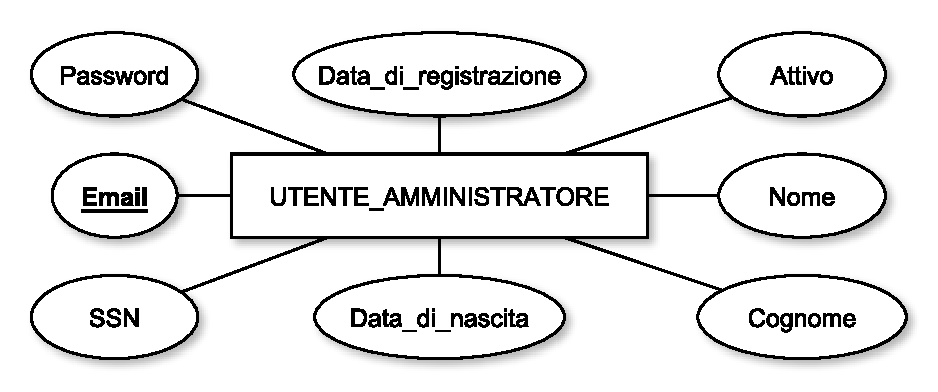
\includegraphics[width=0.8\textwidth]
		{immagini/01-utente-amministratore}
		
		\caption{Entità Utente Amministratore}
	\end{figure}	
	
	\subsubsection*{Descrizione Attributi}
	
	\begin{description}
		
		\item[Id]
		Chiave primaria dell'entità che identifica univocamente il prodotto. Il valore di tale attributo viene generato mediante un contatore.
		
		\item[Data inserimento]
		Chiave primaria dell'entità che identifica univocamente il prodotto. Il valore di tale attributo viene generato mediante un contatore.
		
		\item[Nome]
		Chiave primaria dell'entità che identifica univocamente il prodotto. Il valore di tale attributo viene generato mediante un contatore.
		
		\item[Descrizione]
		Chiave primaria dell'entità che identifica univocamente il prodotto. Il valore di tale attributo viene generato mediante un contatore.
		
		\item[Disponibilita]
		Chiave primaria dell'entità che identifica univocamente il prodotto. Il valore di tale attributo viene generato mediante un contatore.
		
		\item[Peso]
		Chiave primaria dell'entità che identifica univocamente il prodotto. Il valore di tale attributo viene generato mediante un contatore.
		
		\item[Prezzo unitario]
		Chiave primaria dell'entità che identifica univocamente il prodotto. Il valore di tale attributo viene generato mediante un contatore.
		
		\item[Immagine]
		Chiave primaria dell'entità che identifica univocamente il prodotto. Il valore di tale attributo viene generato mediante un contatore.
		
	\end{description}
	
	\subsection{Utente Amministratore}
	
	\subsection{Utente Registrato}
	
	\subsection{Ordine}
	
	\subsection{Pagamento}
	
	\subsection{Fattura}
	
	\subsection{Ricetta}
	
	\subsection{Marchio}
	
	\subsection{Caratteristica}
	
	\subsection{Reparto}
		
	\subsection{Coupon}

\section{Descrizione delle associazioni}

\section{Il modello E-R completo}
\begin{figure}[h]
	\centering
	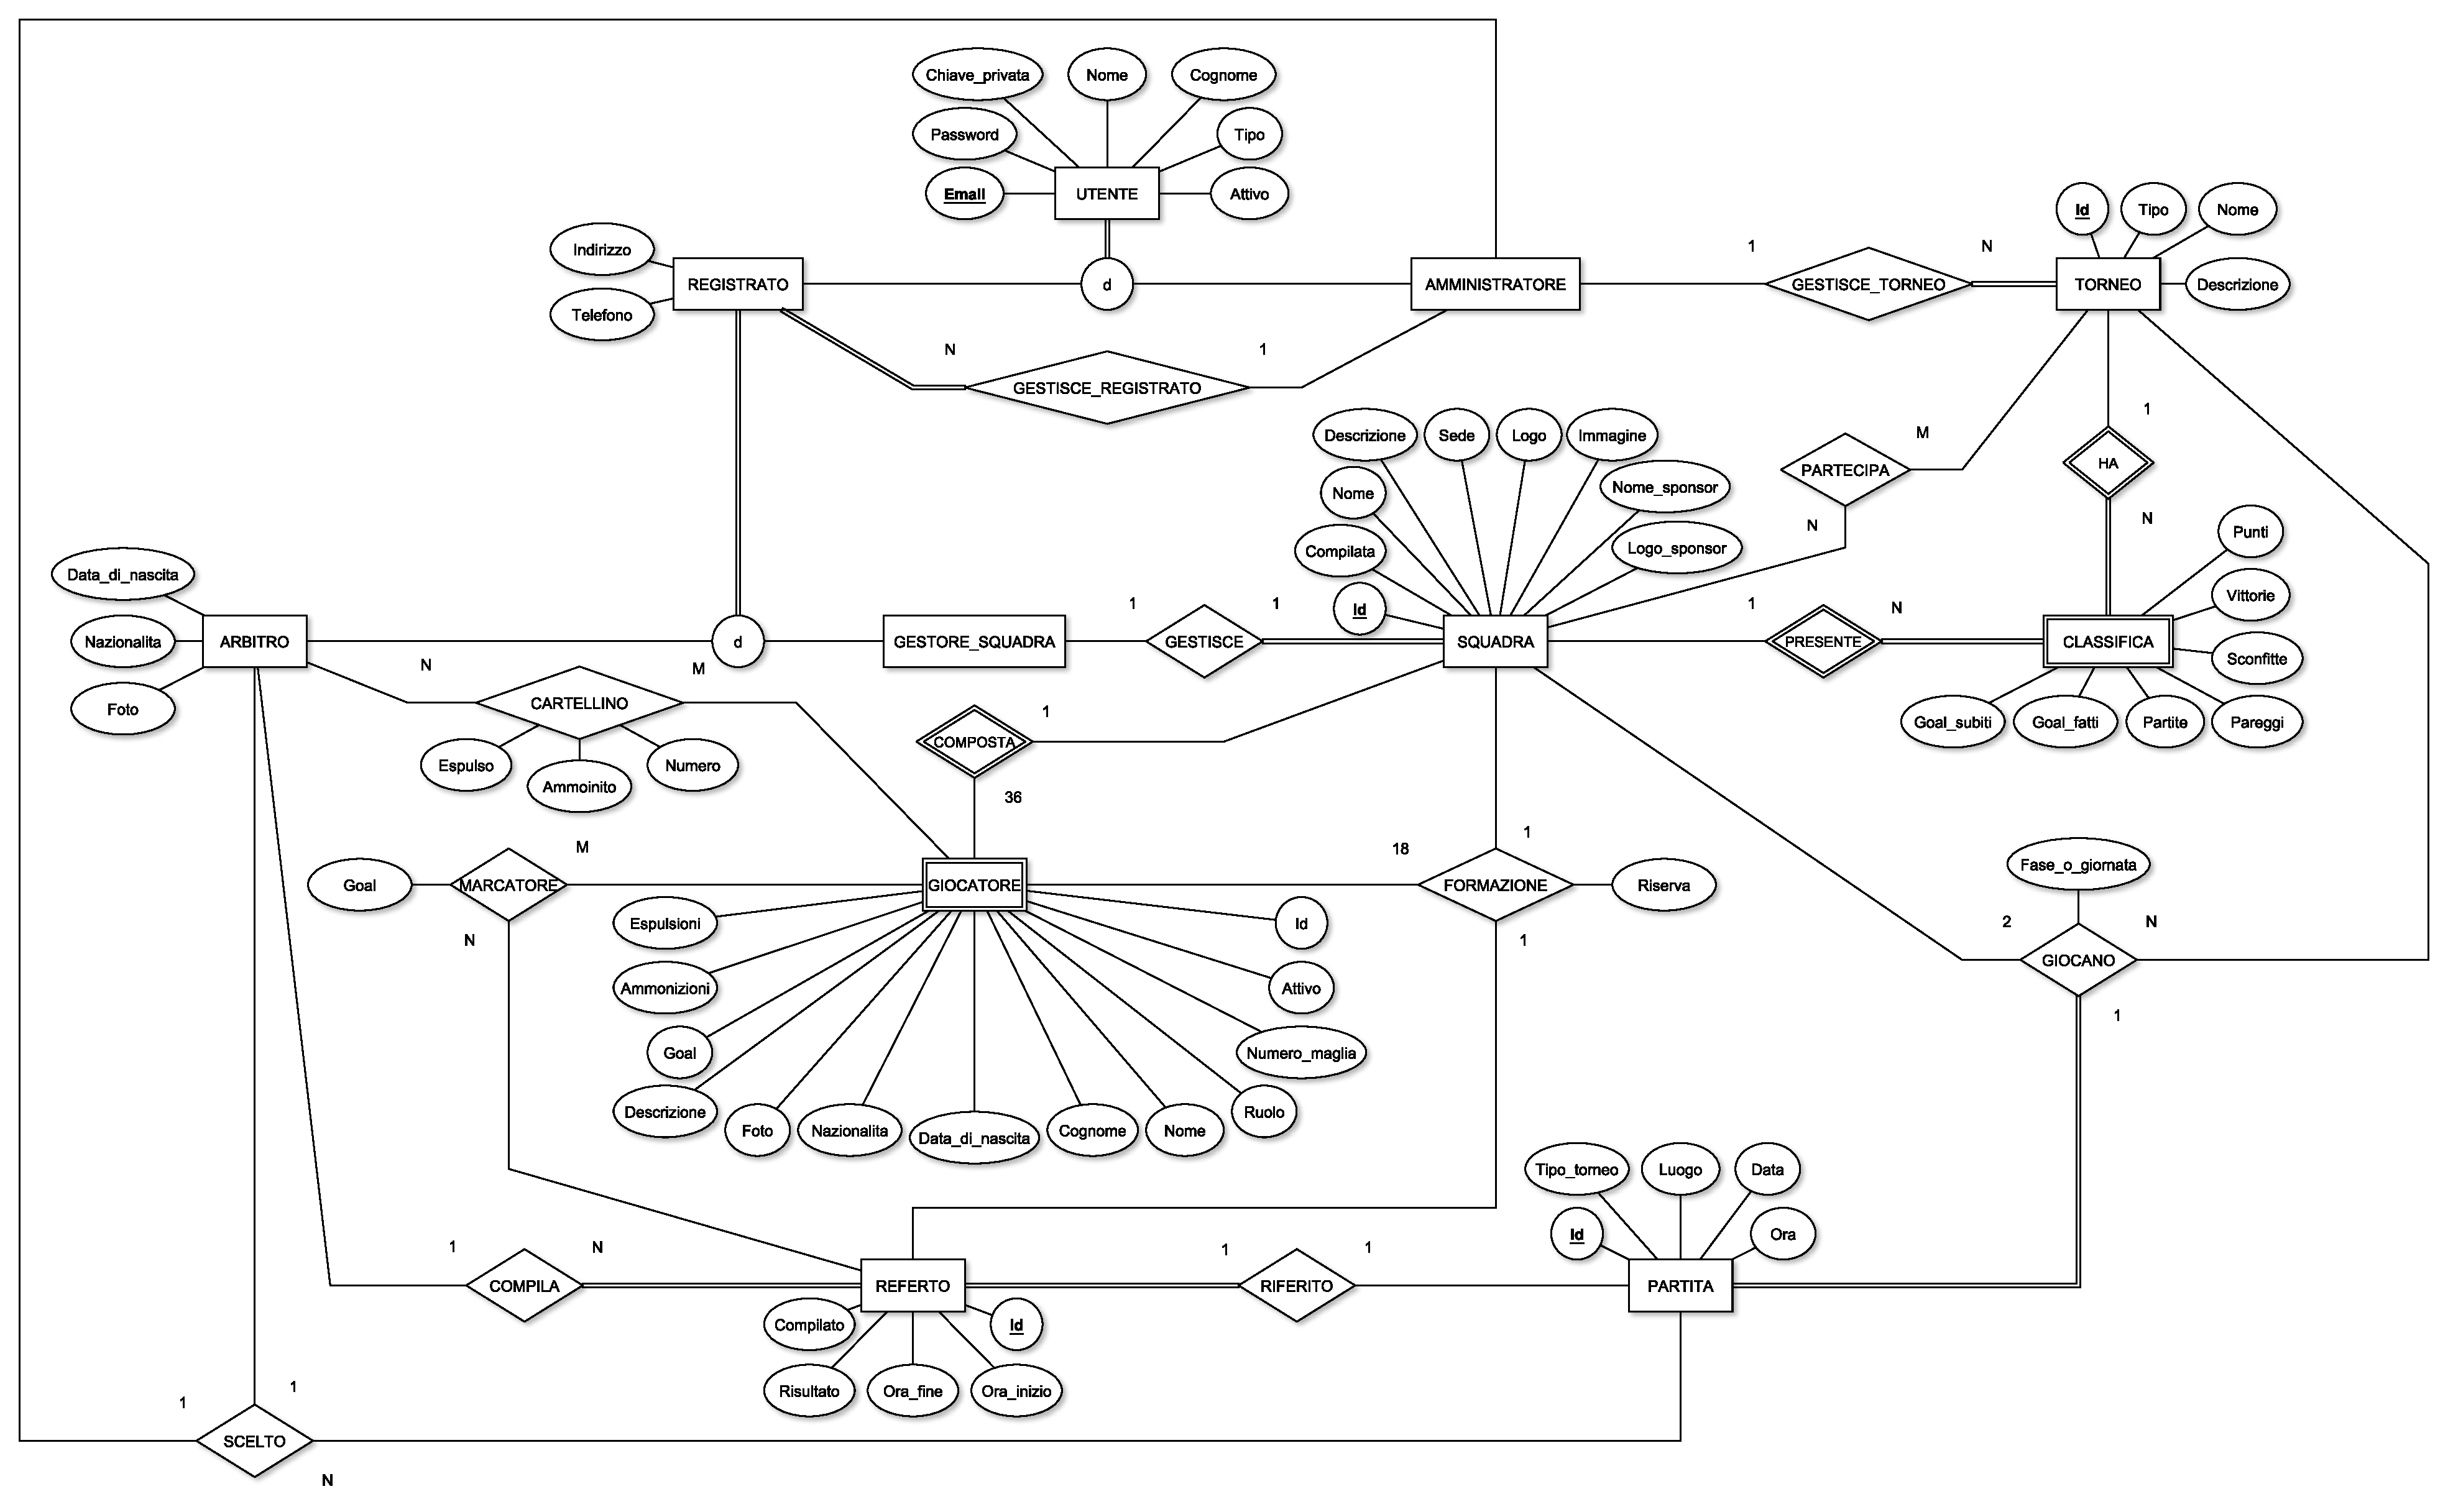
\includegraphics[width=1\textheight,
	angle=90]
	{immagini/diagramma-ER-completo}
	
	\caption{Schema E-R completo}
\end{figure}	